\documentclass{beamer}
\usetheme{Antibes}
\useinnertheme{rectangles}
\useoutertheme{infolines}
\usepackage[utf8]{inputenc}
\usepackage[T1]{fontenc}
\usepackage[ngerman]{babel}

% patch the look of +, = in arev
\usefonttheme{serif} 

\usepackage{arev}
\usepackage{amsmath}
\usepackage{amssymb}
\usepackage{graphicx}
% \setbeamertemplate{caption}[numbered]

\setbeamertemplate{footline}{%
\begin{beamercolorbox}[ht=3.0ex,dp=1ex]{title in head/foot}
\hfill\footnotesize\insertpagenumber\enspace\enspace\end{beamercolorbox}}

\newcommand{\ee}{\mathrm e}
\newcommand{\ui}{\mathrm i}
\newcommand{\real}{\operatorname{Re}}
\newcommand{\imag}{\operatorname{Im}}
\newcommand{\uv}[1]{\underline{#1}}
\newcommand{\bv}[1]{\mathbf{#1}}

\newcommand{\N}{\mathbb N}
\newcommand{\Z}{\mathbb Z}
\newcommand{\Q}{\mathbb Q}
\newcommand{\R}{\mathbb R}
\newcommand{\C}{\mathbb C}

\newcommand{\id}{\operatorname{id}}
\newcommand{\sgn}{\operatorname{sgn}}
\newcommand{\Abb}{\operatorname{Abb}}
\newcommand{\unit}[1]{\mathrm{#1}}
\newcommand{\chem}[1]{\mathrm{#1}}
\newcommand{\strong}[1]{\textsf{\textbf{#1}}}

\newcommand{\imgcaption}[1]{{\small #1}}

\title{Die Peano-Axiome}
\subtitle{Die natürlichen Zahlen als dynamisches System}
\date{}

\begin{document}
\renewcommand*{\figurename}{Abb.}

\begin{frame}

\maketitle

\end{frame}

\begin{frame}
Wir haben zunächst eine beliebige Menge $N$ die als $N\subseteq\Omega$
in die Grundmenge (das Universum) $\Omega$ eingebettet sein soll.\\[1em]

Außerdem haben wir eine Abbildung $s\colon N\to\Omega$.\\[1em]

Einmal später sollen $N$ die natürlichen Zahlen sein und $s$ die
Nachfolgerfunktion $s(x):=x+1$. Diese Vorstellung wollen wir zunächst
vergessen, zunächst sind $N$ und $s$ völlig beliebig.
\end{frame}

\begin{frame}
Als erstes legen wir fest, dass für jedes $x\in N$ auch $s(x)\in N$
sein soll. Anders ausgedrückt heißt das, dass $s\colon N\to N$ ist,
dass es sich bei $s$ also um eine Selbstabbildung handelt.\\[1em]

Bei einer iterierten Selbstabbildung handelt es sich um ein dynamisches
System. Von einem Startwert (Anfangszustand) $x$ aus können wir den Orbit
\[\{x,s(x),s(s(x)),s(s(s(x))),\ldots\}\]
bilden.
\end{frame}

\begin{frame}
Es ist aber schon gesagt, dass $s$ eine Abbildung ist. Damit ist jedem
$x\in N$ genau ein $s(x)$ zugeordnet. Eine Trajektorie (ein Orbit)
kann sich niemals an einer Stelle verzweigen, weil es immer nur
ein $s(x)$ geben kann.
\end{frame}

\begin{frame}
\begin{center}
\includegraphics[width=0.5\textwidth]{img/Nichtinvertierbares-System.pdf}
\end{center}
\imgcaption{Es kann bis jetzt aber sein, dass das System aus zwei
unterschiedlichen Vergangenheiten in den selben Zustand mündet.}
\end{frame}

\begin{frame}
\begin{center}
\includegraphics[width=0.4\textwidth]{img/Zyklische-Zukunft.pdf}
\end{center}
\imgcaption{Dazu gehört auch die Einmündung in einen Zyklus.}
\end{frame}

\begin{frame}
Um das zu unterbinden, legen wir fest, dass $s$ injektiv sein soll.
Das heißt
\[\forall x,y\; (s(x)=s(y)\implies x=y).\]
\end{frame}

\begin{frame}
Als nächtes wollen wir, dass es einen Zustand $0\in N$ gibt, dass es
also eine Trajektorie gibt, die durch $0$ verläuft.
\end{frame}

\begin{frame}
Bis jetzt sind zyklische Systeme nicht verboten, so dass es einen
endlichen Orbit gibt, und irgendwann $s(x)=0$ ist. Oder die Trajektorie
kommt aus einer unendlichen Vergangenheit bis man $s(x)=0$ erhält.
\end{frame}

\begin{frame}
\begin{center}
\includegraphics[width=0.4\textwidth]{img/Zyklisches-System.pdf}
\end{center}
\imgcaption{Systeme mit unendlicher Vergangenheit und
zyklische Systeme sind bis jetzt nicht verboten.}
\end{frame}

\begin{frame}
Wir unterbinden das ganz banal mit der folgenden Festlegung:
\[\forall x\;(x\in N\implies s(x)\ne 0).\]
\end{frame}

\begin{frame}
Das letzte und schwierigste Problem, das uns Sorgen bereitet, ist
das der »Parallelstrukturen«. Damit ist folgendes gemeint.
Es kann neben $\operatorname{Orbit}_s(0)$
weitere Trajektorien geben. Die können
\begin{itemize}
\item irgendwo aus einer Quelle entspringen und in die unendliche Zukunft laufen,
\item aus einer unendlichen Vergangenheit kommen und in die unendliche Zukunft laufen,
\item zyklisch sein.
\end{itemize}
\end{frame}

\begin{frame}
Diese parallelen Geschichten haben zwar mit
$\operatorname{Orbit}_s(0)$ nichts zu tun, können aber vorhanden sein.
\end{frame}

\begin{frame}
\begin{center}
\includegraphics[width=0.4\textwidth]{img/Parallelstrukturen.pdf}
\end{center}
\imgcaption{Die natürlichen Zahlen und mögliche Parallelstrukturen, die bis jetzt
mit ihnen koexistieren können.}
\end{frame}

\begin{frame}
Wir wollen eigentlich, dass jeder Zustand in einer endlichen Zahl
von Schritten von $0$ aus mit $s$ erreicht werden kann.
\end{frame}

\begin{frame}
Wir könnten einfach den Orbit definieren:
\[\operatorname{Orbit}_s(0) := \{s^k(0)\mid k\in\N\}\]
mit
\[s^0(x):=x,\quad s^{k+1}(x):=s(s^k(x)).\]
Die natürlichen Zahlen, deren Struktur wir definieren wollen,
kommen jetzt aber in der Definition vor. Die Definition ist
somit leider zirkulär. Wir müssen anders argumentieren.
\end{frame}

\begin{frame}
Wenn $M\subseteq\N$ ist und null enthält, dann gibt es doch
eine Zahl $x$ mit $x\in M$ und $x+1\notin M$. Anschaulich heißt das,
dass das System irgendwann aus $M$ ausbricht.
\end{frame}

\begin{frame}
\begin{center}
\includegraphics[width=0.6\textwidth]{img/Teilmengen.pdf}
\end{center}
\end{frame}

\begin{frame}
Allgemeiner ist bei $\N\not\subseteq M$ ein Ausbruch aus $M$ möglich.
\end{frame}

\begin{frame}
Betrachten wir nun also ein $M$ mit $0\in M$ und $N\not\subseteq M$.\\[1em]

Angenommen $N$ enthält nun Parallelstrukturen, und $M$ sind die
eigentlichen natürlichen Zahlen. Dann ist $0\in M$ richtig. Auch
$N\not\subseteq M$ ist der Fall, genauer $M\subseteq N$.\\[1em]

Wir können aber kein $x$ mit $x\in M$ und $s(x)\notin M$ finden.
Wären $N$ die echten natürlichen Zahlen, dann wäre das nach
unseren letzten Überlegungen unmöglich.
\end{frame}

\begin{frame}
Das soll für jede beliebige Menge $M$ mit $N\not\subseteq M$ und
$0\in M$ gelten. Wir fordern also:
\[\forall M\; (N\not\subseteq M\land 0\in M\implies
\exists x{\in}N\;(x\in M\land s(x)\notin M)).\]
Ohne unsere vorherige Überlegung ist diese Formel mental anspruchsvoll.
Das wird nicht besser nachdem wir die Formel einigen logischen
Umformungen, einschließlich Kontraposition, unterzogen haben. Als
äquivalente Formel ergibt sich die klassische Form des letzten Peano-Axioms:
\[\forall M\; (0\in M\land
\forall x{\in}N\;(x\in M\implies s(x)\in M)\implies N\subseteq M).\]
\end{frame}

\begin{frame}
Man kann jetzt die Addition und die Multiplikation rekursiv
definieren. Für die Funktion $s$ gilt dann $s(x)=x+1$.\\[1em]

Die Struktur der natürlichen Zahlen müsste durch ein dynamisches System
$(N,s)$, welches die genannten Axiome erfüllt,
eindeutig charakterisiert sein.\\[1em]
\end{frame}

\begin{frame}
Ende.
\end{frame}

\end{document}


